% !TEX root = main.tex

\subsection{Heterogeneous-Aware Channel Evaluation}
\label{sec:hce}
\label{sec:metric}

With our hypergraph-based model of the environment, we can represent which radios and links coordinate or interfere with each other. In today's highly dense environments, entirely separating such networks in the spectrum is unlikely.  Instead, such networks need to be intelligently placed (often overlapping) so as to minimize their interference.  Performing intelligent placement requires the ability to estimate performance across many possible channels.  Prior work has only directly measured interference of heterogeneous radios on WiFi~\cite{wifinet}, leveraging loss information provided by WiFi radios.  The work is unable to \emph{estimate} interference if placed at a different frequency, and the work does not consider interference as many-to-many: it only considers many-to-WiFi.

In this section, we discuss the basis for estimating the performance of a network/radio on a different channel under heterogeneous conditions (\S\ref{sec:deriveest}), the impact traffic workloads can have (\ref{sec:workloads}), how to estimate overlap and loss (\S\ref{sec:sigma}), and finally the accuracy of such a metric (\S\ref{sec:verifysigma}). 

\subsubsection{Basis for a Heterogeneous Channel Estimate}
\label{sec:deriveest}

Predicting performance on another channel in a homogeneous environment can be estimated by calculating expected airtime on a channel~\cite{whitefi}, which is the maximum of:  1) The residual airtime when operating at center frequency $f$, and 2) The expected fair-share operating at a frequency of $f$, given $B_{f}$ nodes currently operating there.  With a residual airtime of $A_f$ at frequency $f$, the expected airtime for radio $r$ is:

%Therefore, the expected airtime for radio $r$ operating at a frequency of $f$, which has a residual airtime of $A_f$, is:

\vspace{-0.15in}
\begin{equation}
\label{eq:homo_airtime} 
\rho_r(f)~=~max(1 - A_f, \frac{1}{B_f + 1})
\end{equation}

\noindent However, in a heterogeneous environment one must also account for a loss in the expected airtime due to \emph{sustained interference}. If the radio sustains interference interference during 30\% of this airtime, then its expected airtime is $\rho_n(f) * 0.7$, since only 70\% of its airtime will be ``useful."

\begin{figure}[t]
\centering
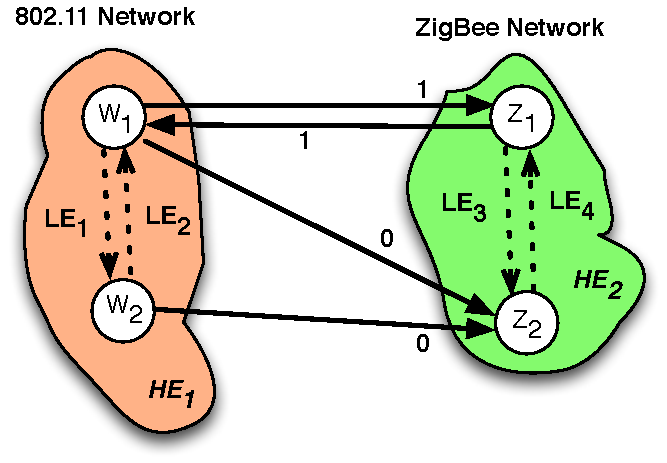
\includegraphics[width=1.8in]{figures/linkexample}
\vspace{-0.2in}
\caption{\label{fig:linkexample} \small Example of heterogeneous interference on links.}
\center
\vspace{-0.1in}
\end{figure}

When we a radio's sustained interference, we focus on the interference sustained on links that the radio acts as the transmitter.  Consider the example illustrated in Figure~\ref{fig:linkexample} with 4 radios and 3 links.  Focusing on $Z_1$'s sustained interference would consider interference on link $LE_3$, \emph{and not} $LE_4$.   The performance of $LE_3$ is dependent on interference at the receiver ($Z_2$) from links whose transmitters do not coordinate with $Z_1$.  Although $Z_2$ is within spatial range of both $W_1$ and $W_2$, $LE_1$ coordinates with $LE_3$ since $W_1$ and $Z_1$ coordinate (i.e., $SE\{Z_1,W_1\}=1$ and $SE\{W_1,Z_1\}=1$).  However, $LE_2$ conflicts with $LE_3$ since $Z_2$ is within spatial range of $LE_2$'s transmitter ($W_2$), which does not coordinate with $Z_1$. 

%Ultimately, we estimate the sustained interference on a radio

%Focusing on radio $Z_1$ and the performance of the links it partakes in as the transmitter

%Therefore, when calculating the expected airtime for a radio (such as $Z_1$ in our example), it is important to ``degrade'' its expected fair share of airtime by sustained interference on its links.  

%, extending Eq.~\ref{eq:homo_airtime}, 

With this understanding, we can derive an expected heterogeneous aware performance of a radio $n$ and its links as follows.  First, $n$ receives its fair share of the airtime from the radios that $n$ is within spatial range of and coordinates with.  We consider these nodes to belong to $C_n(f)$ and, referencing our model (\S\ref{sec:model}), are either connected to $n$ via a hyperedge (i.e., they belong to the same network), or with a uni-directional edge \uline{from} $n$ with a weight of 1 (i.e., $n$ coordinates with them).  Then, we degrade this expected fair share by $\sigma^n_f$, an estimate of the sustained interference that each of $n$'s links will experience due to uncoordinated radios:

\vspace{-0.1in}
\begin{equation}
\label{eq:hce}
 hce_f(n) = max(1 - \hspace{-0.12in} \sum\limits_{n_k \in C_n(f)} \hspace{-0.1in} A_f^{n_k}, \frac{
% \hspace{0.05in} \sum\limits_{n_k \in s_n(c)} \hspace{-0.1in} A_c^{n_k}
 1
 }{|C_n(f)| + 1})*(1-\sigma{\hspace{0.015in}_{f}^{n}})%-(1-\gamma{\hspace{0.02in}_{c}^{n}})~~
 \end{equation}

\textbf{The Challenge:} Clearly, the challenge is estimating $\sigma^n_f$, which is a contribution of our work.  There are two components which contribute to $\sigma^n_f$:  1) \emph{Traffic workloads} that vary how often two heterogeneous radio's transmissions will overlap, and 2) A \emph{loss rate} on the links when transmissions do overlap. 

%In the remainder of this section, we discuss  In line with the goals of our work, $\sigma^n_f$ must be estimated in a generic way towards longevity of our model, and is the focus of the remaining sections.

%In the remainder of this section, we describe how to estimate sustained interference towards better heterogeneous spectrum management (\S\ref{sec:sigma}), and show that such an estimate is accurate in (\S\ref{sec:sigma_eval}). 

\subsubsection{The Impact of Traffic Workloads}
\label{sec:workloads}

 The impact of workloads


%When the observed airtime $A_c$ is low, the expected airtime is the residual airtime on the channel: $1 - A_c$.  When airtime utilization is high, the expected airtime is the \emph{fair share} under channel contention: $1 / (B_c + 1)$. 

%While such a metric works well for channel selection and planning in homogeneous environments, it fails to account for two prominent factors within heterogeneous environments:  1) \emph{sustained interference:} a loss of expected airtime due to sustained heterogeneous network interference, and 2) \emph{generated interference}: the amount of interference the network being deployed creates on other networks in the channel.   Clearly, both can have a significant impact on the network joining the channel and those already using the channel.
%
%Taking these factors in to consideration during channel selection and planning is a challenge.  First, distributedly, networks have difficulty detecting and scanning for heterogeneous networks in the spectrum to estimate the interference factors.  Second, even with the knowledge of network spectrum locations (e.g., provided by the Home Spectrum Broker), %how to estimate both factors without requiring the network to ``try'' each channel to evaluate interference on the networks is non-trivial.  In this section, we present a method to estimate both
%a straw man approach such as``trying'' channels to measure both factors of interference would be complex and time-consuming.  
%
%In this section, we present a novel \emph{Heterogeneous-Aware Channel Evaluation} (HCE) metric which includes both factors of interference to perform intelligent channel selection and planning.  Leveraging basic information at the spectrum broker (airtime utilization and spectrum placement), we find that we can accurately estimate interference between networks by modeling them as independent processes which generate events (i.e., transmissions) based on their airtime utilization.  Using the metric, which provides an expect ``channel quality,'' we can: 1) guide a network to an appropriate channel to minimize sustained and generated interference given a set of networks in the spectrum, and 2) perform an optimal ``planning" of networks, given a  set of networks that are non-configurable while also accounting for network restrictions (e.g., network contains a 2.4GHz only device). 

%\subsection{Heterogeneous Channel Evaluation (HCE)}
%
%The \emph{heterogeneous channel evaluation} (HCE) metric represents an estimated ``channel quality'' for a network $n$, in channel $c$, denoted as: $hce_c(n)$.  HCE takes in to consideration the airtime of the channel, as well as heterogeneous interference sustained ($\sigma_c^n$) and generated ($\gamma_c^n$).   For discussion below, we present the derivation of HCE in Equation~\ref{eq:hce}. 
% 
% \begin{equation}
%\label{eq:hce}
% hce_c(n) = \rho_n(c)*(1-\sigma{\hspace{0.015in}_{c}^{n}})-(1-\gamma{\hspace{0.02in}_{c}^{n}})~~
% \end{equation}
%
%
%Shown in Equation~\ref{eq:homo_airtime}, the residual airtime in a homogeneous environment is a function of the total airtime: 1 - $A_c$.      In a heterogeneous environment, the expected residual airtime (independent of interference) for a network $n$ on channel $c$ is a function of the airtime of the set of networks that $n$ can sense on $c$:  $s_n(c)$.  Networks that $n$ cannot sense on $c$ will instead contribute to the amount of sustained interference ($\sigma_c^n$).   Therefore, residual airtime is 1 minus the sum of airtime of networks in $s_n(c)$, shown Equation~\ref{eq:hce}. 
%
%While network $n$ can expect a fair share of airtime, this fair share is only expected from the set of networks that coordinate with $n$.  Meaning, a set of networks that can sense $n$, and $n$ can sense such networks.  We define this set of coordinating networks on channel $c$ with respect to network $n$ as: $d_n(c)$.  We can estimate this fair-share of airtime by taking the total airtime of coordinating networks, and dividing it by the number of nodes, including network $n$: $|d_n(c)| + 1$.   Note that we do not use the reciprocal of $|d_n(c)| + 1$, as in Equation~\ref{eq:homo_airtime}, since we need to account for only the airtime used by coordinating networks.  Equation~\ref{eq:homo_airtime} assumes all networks coordinate, therefore the sum of their possible airtime is 1.  
%
%The maximum of the residual airtime and the fair-share is the expected airtime, independent of interference.  In the remainder of this section, we present the estimated \emph{loss} of this expected airtime due to sustained interference ($\sigma_c^n$), and a channel quality deduction due to generated interference ($\gamma_c^n$).

\subsubsection{Estimating Heterogeneous Interference ($\sigma^n_f$)}
\label{sec:sigma}

To estimate the sustained heterogeneous interference of radio $n$'s links operating at a frequency $f$ from non-coordinating radios (within interference range of its link's receivers), we leverage the following key observation.  Without being able to sense each other, \emph{heterogeneous radios operate entirely independently.}  As a result, their events (i.e., packet transmissions) occur continuously and independent of one another.  Therefore, heterogeneous radios can be modeled as independent Poisson processes in which, using knowledge of their average transmission lengths and airtimes, we can estimate their probability of overlapping transmissions.  This allows us to estimate sustained interference between non-coordinating radios on a frequency $f$ to derive $\sigma^n_f$.  This derivation is similar to historical estimations of collisions in Ethernet networks without CSMA, as the underlying behavior (inability to coordinate) is the same.  

\vspace{0.1in}
\noindent \uline{Primer:} Given a radio $j$ with an average transmission rate of $\lambda_j$ (based on its airtime usage), the probability of $K$ transmissions from the radio $j$ in a time window of $T$ is:

\vspace{-0.15in}
\begin{equation}
\label{eq:poisson}
P(K,T)~=~\frac{(\lambda_j T)^K~~e^{- \lambda_j T}}{K!}
\end{equation}
%\vspace{0.01in}

\noindent Likewise, the probability zero transmissions from radio $j$ in a time window of $T$ is:

\vspace{-0.15in}
\begin{equation}
\label{eq:zero}
P(K_j=0,~T)~=~\frac{(\lambda_j T)^0~~e^{- \lambda_j T}}{0!}~=~e^{- \lambda_j T}
\end{equation}

\noindent And, important to our derivation, the probability of \emph{any} transmission from $j$ in window $T$ is the complement of zero transmissions from $j$ in $T$:

\vspace{-0.15in}
\begin{equation}
\label{eq:any}
P(K_j>0,~T)~=~1-e^{- \lambda_j T}
\end{equation}

\vspace{0.1in}
\noindent \uline{Estimating Overlap From a Single Radio:}  Building towards our estimate of sustained interference on $n$'s links, we can use these calculations to estimate the probability a single heterogeneous (i.e., independent) radio $j$ within interference range of $n$'s receiver $r$ will overlap with transmissions on the link $LE\{n,r\}$.  This would be the probability of any transmission from $j$ within a vulnerability window for a transmission from $n$ to $r$,  denoted $V^{nr}_j$ (i.e., $P(K_j>0,~V^{nr}_j)$).  The length of this window is dependent on whether both transmitters do not coordinate with each other, or whether at least one transmitter coordinates.  If both do not coordinate, the average vulnerability window is the sum of $j$ and $n$'s average transmission lengths: $V^{nr}_j = t_j + t_n$. However, if $n$ coordinates with $j$ (i.e., $n$ can sense $j$'s transmissions, but not visa-versa), then the vulnerability window is reduced to $V^{nr}_j = t_n$.  

\begin{figure}[t]
\centering
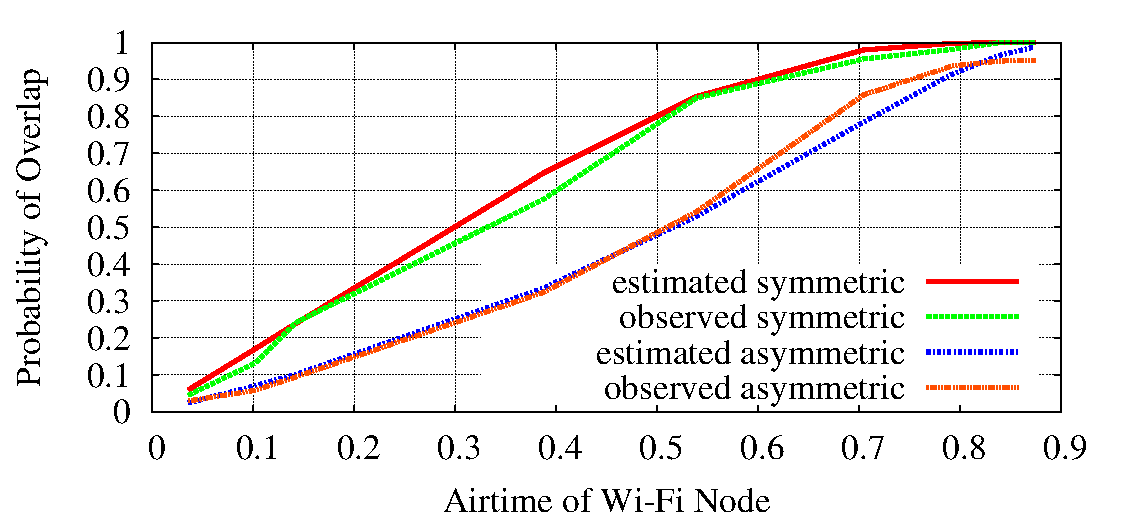
\includegraphics[width=3in]{figures/eo_overlaps_both}
\vspace{-0.2in}
\caption{\label{fig:overlap} \small The probability of overlapping transmissions.}
\center
\vspace{-0.1in}
\end{figure}

%This is because, in the prior case, $n$ may start a transmission within a transmission from $j$ (since it cannot sense it), whereas in the latter case it cannot (since $n$ will sense $j$'s transmission). 


%To estimate the amount of sustained interference from heterogeneous radio $j$ on the radio $n$ (i.e., probability of loss due to $j$), we want to know the probability of \emph{any} events (i.e., transmissions) from $j$ within in a transmission from $n$'s vulnerability window $T^n_j$ .  In other words, the probability of a transmission from $j$ during a transmission from $n$ (a packet is vulnerable throughout its duration). This can be done by calculating the complement  of zero events in the vulnerability window $T^n_j$:


%Estimating the amount of sustained interference from this network $j$ (i.e., probability of loss due to it) can be made by first calculating $P(K=0,T)$: the probability of no transmissions in a vulnerability time window of T, thereby the estimated success rate of transmissions under interference from network $j$.  

This reasoning for this is best described by referring back to our example model in Figure~\ref{fig:hypergraph}.  The edges labeled $A$ show a ZigBee radio that is close enough to a WiFi radio to result in $Z_1$ coordinating with $W_1$ (i.e., E\{$W_1$, $Z_1$\}=1), however the ZigBee radio (despite spatially overlapping with the WiFi radio) is not powerful enough to cause $W_1$ to back-off (i.e., E\{$Z_1$, $W_1$\}=0).  This means that $Z_1$ will be able to sense $W_1$'s transmissions and back-off to them, meaning $Z_1$'s vulnerability from $W_1$ is only during the length of one of $Z_1$'s transmissions.  If the situation was ``double-blind," then the vulnerability window increases by the length of $W_1$'s transmission length, since in this situation $Z_1$ would not be able to sense them and accidentally transmit during them. 

Therefore, the probability of \emph{any transmission} from node $j$ within the respective vulnerability window for link $LE\{n,r\}$ would be derived from Equation~\ref{eq:any} as:

\vspace{-0.15in}
\begin{equation}
\label{eq:overlap_single}
P(K_j>0,~V^n_j)~=~1-e^{- \lambda_j V^{nr}_j}
\end{equation}

\vspace{0.1in}
\noindent \uline{Estimating Overlap From Any Uncoordinated Radio:}  Estimating the probability of overlap on $LE\{n,r\}$ from \emph{any} uncoordinated radio in the environment within range of $n$'s receiver $r$ is similar in nature.  Again, we want to take the compliment of the probability of zero transmissions during a transmission from $n$.  In an environment with multiple uncoordinated radios, the probability of zero transmissions would be the product of the probabilities of zero transmissions from each uncoordinated radio.  We consider these radios to be the intersection of the sets $U_n(f)$ and $S_r(f)$.  That is, the radios that do not coordinate with the transmitter $n$ (i.e., $U_n(f)$) that are also within spatial range of the receiver $r$ (i.e., $S_r(f)$).  Referring to our hypergraph-based model, radios in $U_n(f)$ are nodes with uni-directional edges \uline{to} $n$ with a weight of 0, and $r$ must also be in spatial range of these radios (i.e., an edge to $r$, regardless of weight).  Therefore, the probability of overlap from any node in $U_n(f) \cap S_r(f)$ during a transmission on $LE\{n,r\}$ would be the complement of zero transmissions from all such radios:

\vspace{-0.15in}
\begin{equation}
\label{eq:overlap_any}
\hat{\sigma}^n_f(LE\{n,r\})~~=~~ 1~~ - \hspace{-0.1in} \prod\limits_{j \in U_n(f) \cap S_r(f)} \hspace{-0.2in}e^{- \lambda_n V^{nr}_j}
 \end{equation}

% due to any transmission from a radio in , which finally derives $\sigma^n_c$, is product of their estimated 
%
%First, we can calculate the probability of zero transmissions from each uncoordinated radio as \emph{the product of the probabilities} of zero
%
% but requires the consideration that there must zero transmissions from all radios in the vulnerability window.  The probability of 

%Next, consider 
%
%The probability of a successful transmission in an environment with multiple un-coordinated radios would be the complement of having zero events from each of these radios in the vulnerability window.  

% $n$ can sense $j$.~\footnote{Network $j$ must \emph{not} sense $n$, otherwise the estimated sustained interference from it is considered to be 0 due to sensing.} If true, the vulnerability window is the average length in time of $n$'s transmissions, denoted $t_{n}$. If false, then the vulnerability window is $t_{n}$ plus the average length of $j$'s transmissions: $t_{j}$. The reason for the latter case is that the transmission is vulnerable throughout its duration ($t_n$), and $t_j$ in time before hand in which if $j$ starts a transmission it will not complete before $n$'s transmission begins.

\vspace{0.1in}
\noindent \uline{Accounting for Loss Rate During Overlap:}  Of course, not all overlaps can create a packet loss.  Prior work has shown that at various levels of interference, the loss rate can vary~\cite{buzzbuzz}.  This information can be provided by an external look-up (i.e., leveraging studies already done), or estimated by the underlying monitoring system (e.g., WifiNet). We consider the probability of loss due to overlap from $j$ on receiver $r$ as $L^j_r$ and can apply such non-deterministic loss to overlapping transmissions from uncoordinated networks as:

%To provide the most accurate estimate of sustained interference, it is important to recognize that not all overlaps in transmissions will create loss. Worst case estimation can be calculated by assuming a loss rate due to overlap of 1, and we will show in \S\ref{sec:plan_eval} that this worst-case estimation can lead to good network placement.  However, we can also account for this in our estimation to approach optimal placement if known. We denote $L_n^j$ as $n$'s loss rate due to overlap of transmissions from $j$.  Therefore, the estimated sustained interference in channel $c$ from network $j$ on $n$ is:

\vspace{-0.1in}
\begin{equation}
\label{eq:sus_single}
\sigma_f^n(LE\{n,r\}) ~= ~1~~ - \hspace{-0.1in} \prod\limits_{j \in U_n(f) \cap S_r(f)} \hspace{-0.2in}e^{- \lambda_n V^{nr}_j} * (1 - L^j_n)
\end{equation}

\begin{figure}[t]
\centering
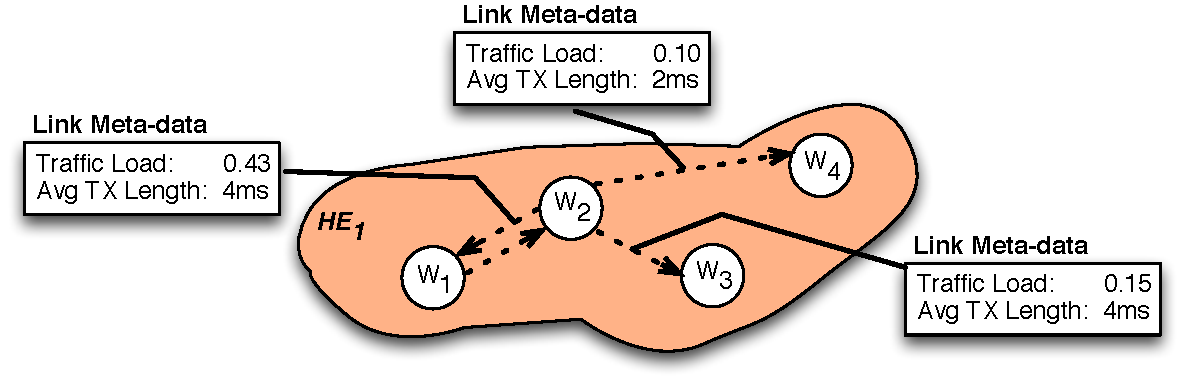
\includegraphics[width=3.2in]{figures/multilink}
\vspace{-0.2in}
\caption{\label{fig:multilink} \small 3 radio and 4 link example used in computing total predicted sustained heterogeneous interference across all links.}
\center
\vspace{-0.1in}
\end{figure}


\begin{figure*}[t]
\centering
\hspace{-0.3in}
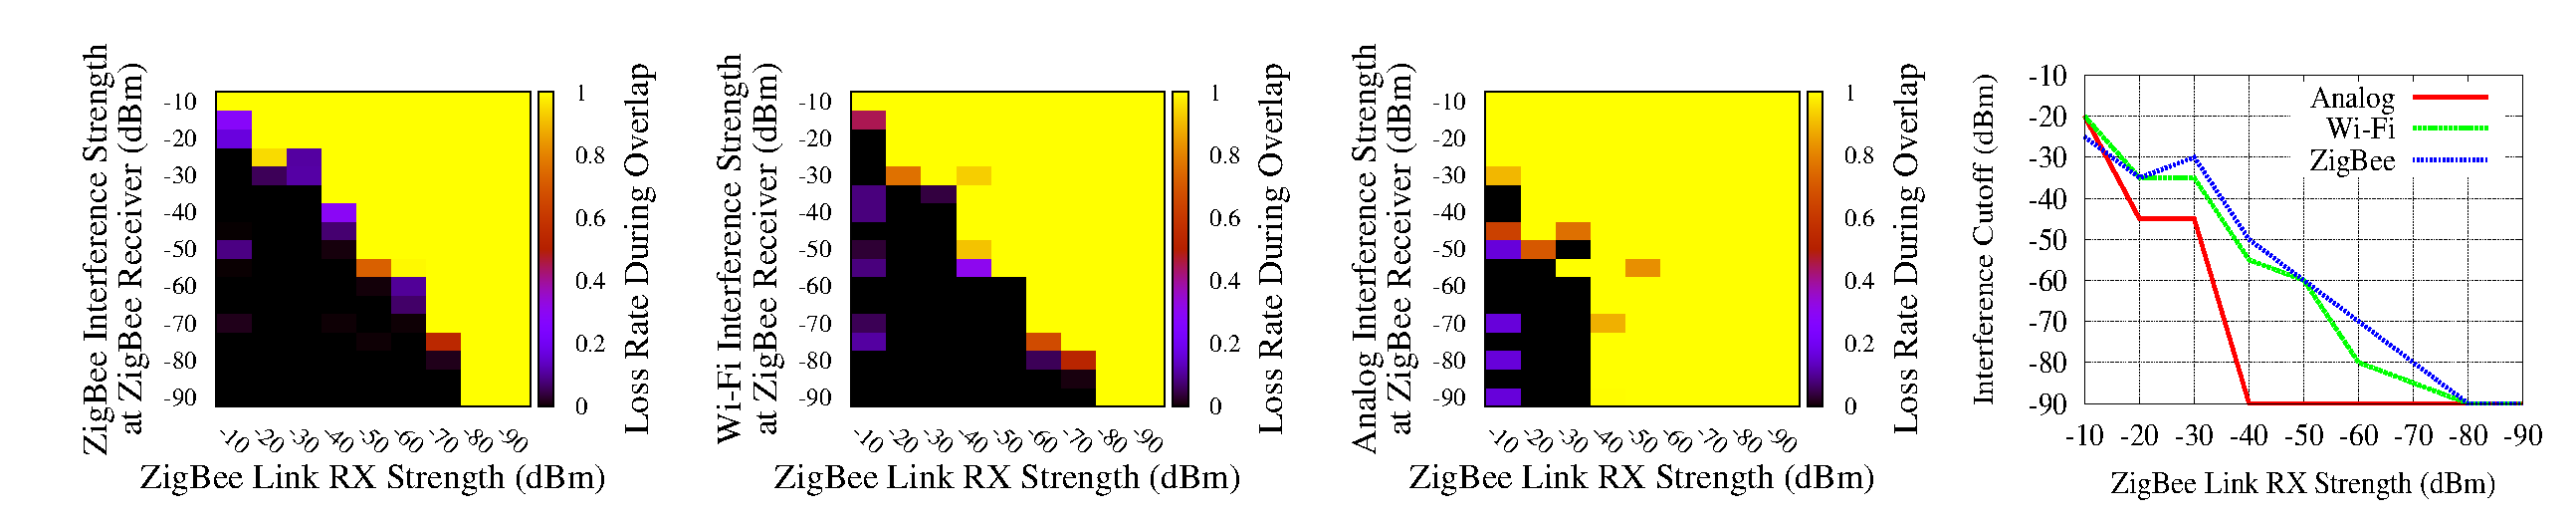
\includegraphics[width=7.2in]{figures/together}
\vspace{-0.2in}
\caption{\label{fig:overlap} \small The probability of overlapping transmissions.}
\center
\vspace{-0.1in}
\end{figure*}

\vspace{0.1in}
\noindent \uline{Total Predicted Sustained Heterogeneous Interference:} Finally, we compute the total predicted sustained heterogeneous interference across all links (i.e., $\sigma^n_f$) as follows.  First, consider the set $L_n$ to contain all of the links that belong to radio $n$. Therefore, referring to Figure~\ref{fig:multilink}:

\vspace{-0.15in}
 $$L_{W_2} = \{~LE\{W_2,W_1\},~LE\{W_2,W_3\},~LE\{W_2,W_4\}~\}$$
 
 \noindent Note that, again, we do not consider $LE\{W_1,W_2\}$ as belonging to $W2$; we consider this link as belonging to $W_1$.  Additionally, we denote the traffic load for the link $LE\{n,r\}$ as $D_{LE\{n,r\}}$, such that $D_{LE\{W_2,W_4\}}=0.10$ in Figure~\ref{fig:multilink}. 
 
 From this, we compute the total predicted sustained interference for a radio $n$ at frequency $f$ as follows:
 
 \vspace{-0.1in}
\begin{equation}
\label{eq:metric}
\sigma_f^n ~= (\sum\limits_{l \in L_n} \sigma^n_f(l) * D_l~) ~~/~ \sum\limits_{m \in L_n} D_m
\end{equation}
 
 \noindent That is, we compute the sum of the sustained interference on each link multiplied by the traffic load on the link, and then divide this sum by the sum of the traffic loads from $n$.   What this provides as a result is the fraction of total airtime it spends that will be lost due to interference.  
 
 Let us consider Figure~\ref{fig:multilink} as a simple example of this computation, focusing on $W_2$.  First, assume all links have a 25\% loss rate, i.e., $\forall ~l \in L_{W_2},~ s^n_f(l) = 0.25$. Therefore, the first summation in Eq.~\ref{eq:metric} becomes:  (.25*.43)+(.25*.10)+(.25*.15) = 0.17. Then, divide this by the right summation and: $\sigma^{W_2}_f = 0.17 / 0.68 = 0.25$ i.e., 25\% of $W_2$'s total airtime is lost due to heterogeneous interference on its links.  Therefore, referencing the reader back to our full predictive measure shown in Eq.~\ref{eq:hce}, $W_2$ would get its fair share (left side of the equation), and this would be scaled down by $1-\sigma^{W_2}_f$, i.e., 1-0.25=0.75 meaning it will only receive 0.75 of its expectation due to heterogeneous interference. 
 
% \vspace{-0.15in}
% \begin{align*}
% \sum\limits_{l \in L_{W_2}} \sigma^{W_2}_f(l) * A(l) &= (.25*.43)+(.25*.10)+(.25*.15) = 0.17 \\
% %&=0.1075 + 0.025 + 0.0375 = 0.17
% \end{align*}
% \vspace{-0.2in}
 
%This provides an estimated loss rate for transmissions by $n$ on frequency $f$ due to sustained heterogeneous interference.  Although a proper $L^j_n$ will provide the most accurate predicted sustained heterogeneous inference, it can be assumed to be 1 (i.e., all overlaps are destructive) if unknown to the monitoring system and the spectrum assignment system.  As we will show, this assumption can still provide good spectrum assignment as it still considers the loads of the networks when calculating predicted interference (\S\ref{sec:eval}).

\subsubsection{Verifying Heterogeneous Interference Estimate}
\label{sec:verifysigma}

Here, we verify that our heterogeneous interference estimate is accurate through simulation and real-world evaluation. 

%Finally, the \emph{total predicted sustained interference} (i.e., $\sigma^n_c$) is the probability of no transmissions from un-coordinated radios during transmissions from $n$.  This would be the product of the probabilities of overlapping with each of these radios, since the resulting scenario desired is the one in which none of these radios are active at the time.  
%
%We consider these radios to belong to the set $h_n(c)$ and, referring to our model again, are nodes with uni-directional edges \uline{to} $n$ with a weight of 0 (e.g., $W_1 \in h_{Z_1}(c)$).  The probability of loss due to any transmission from a radio in , which finally derives $\sigma^n_c$, is product of their estimated 
%
%%From this, the total sustained interference in a channel can be estimated for a network $n$: $\sigma_c^n$, where $\hat{h}_n(c)$ is a set of networks which cannot sense $n$ in channel $c$:
%
%\vspace{-0.1in}
%\begin{equation}
%\label{eq:sus}
%\sigma_c^n ~= \prod\limits_{j \in h_n(c)} (1-e^{- \lambda_j T})~*~L_n^j
%\end{equation}

%\subsubsection{Generated Heterogeneous Interference Estimate}
%
%Generated interference is included as a ``penalty'' on the network's HCE value for a channel.     As shown in Equation~\ref{eq:hce}, the complement of the amount of generated interference is included (1-$\gamma_c^n$).  Therefore, the more interference the network would generate on other networks by joining the channel, the more heavily the HCE value is reduced. If the network would generate zero interference on other networks, there is no reduction in the HCE value.  
%
%Estimating the amount of generated interference from a network joining a channel on all other networks operating in that channel, is calculated similarly to sustained interference.  Consider $h_n(c)$ the set of networks which $n$ cannot sense.  From this, the estimated generated interference from network $n$ on all networks that it cannot sense, is:
%
%\vspace{-0.1in}
%\begin{equation}
%\label{eq:gen}
%\gamma_c^n ~= \prod\limits_{j \in h_n(c)} (1-e^{- \lambda_n T_j})~*~L_j^n * A_c^j
%\end{equation}
%
%Note that it is important to use network $n$'s expected transmission rate ($\lambda_n$).  This penalty is also scaled by the airtime utilization of $j$: $A_j^n$.  The higher the airtime utilization of the opposing network, the higher the penalty for interfering with the network (reducing HCE).  An expected loss due to overlap on $j$'s transmissions from overlap with network $n$ can be specified with $L_j^n$, or set equal to 1 for worst-case analysis.

%Given completely independent networks (neither can sense each other), the vulnerability window of a transmission due to network $j$ is the 
%
%The probability of no events ($K=0$) in window $T$, represents the probability of no transmissions from network $j$ in the time window.  This can be used to estimate the probability of a transmission from another network in the channel not overlapping with a transmission from network $j$.  The time window $T$ is a vulnerability window, in which an event from the opposing network will cause an overlap.  


%\  {Expected Airtime in a Heterogeneous Environment}



%$$ hce_c(n) = max(1 - \hspace{-0.12in} \sum\limits_{n_k \in s_n(c)} \hspace{-0.1in} A_c^{n_k} * \hspace{-0.07in} \prod\limits_{n \in h_j(c)} \hspace{-0.07in} \sigma_{n}^{h_j}), \frac{})$$




%expected airtime under heterogeneous environments since it does not account for a fraction of the airtime being lost due to heterogeneous network interference.  We label such interference as  For example, a channel may have 65\% residual airtime for network $n_2$, given a single other network $n_1$ utilizing 35\% of the airtime.   However, in attempting to utilize this 65\% residual airtime, $n_2$ may experience a 40\% reduction (useful airtime now 39\%), due to interference from $n_1$ and $n_2$ being unable to detect each other's transmissions.
%
%While this increases the accuracy of expected airtime, it still does not account for the network \emph{creating} interference on other networks in the channel.  Thereby reducing performance in the channel.  
%
%%Assuming a homogeneous set of wireless networks, prior work~\cite{whitefi} has shown airtime utilization can be used by a network for channel selection by calculating an \emph{expected share}.  
%%
%%
%%% can blah sense blah, if not then factor in interference
%%
%%% such airtime utilization is not computable on other nodes, but is on HSB
%%While such an estimation is fine to select an "optimal" channel to operate on, maximizing the network's airtime, it assumes
%
%Estimate the loss created by the lack of coordination between the networks.  Given the lack of coordination (e.g., lack of sensing), the two networks operate independently.   From this, we can model the networks as two independent processes Poisson processes to estimate the interference between them.  Since the sum of $N$ independent Poisson processes is a Poisson process, we can model the interference from all devices and all networks of a single protocol, as a single process.  Ultimately, deriving the an estimated amount of interference from the airtime of two operating sets of networks (e.g., 802.11 networks \& ZigBee networks).  Ultimate: want to know the probability of a transmission during the length of our transmission, thereby creating a loss.  We will further extend this to include the fact that not all overlaps contribute to a loss.
%
%To derive this estimated loss, we are able to model the interfering network as a Poisson process.  
%
%This can be done by only knowing Probability of $k$ events in time $T$.  
%
%\vspace{-0.1in}
%$$P(k,T)~=~\frac{(\lambda T)^k~e^{-\lambda T}}{k!}$$
%
%We want to know the probability of an event (i.e., a packet transmission) during a period of time considered the transmission's \emph{vulnerability window}, in which an event would be cause overlap a period of overlap. Therefore, we can calculate this by taking $1- P(k=0)$:
%
%\vspace{-0.1in}
%$$1-P(k=0)~=~1-\frac{(\lambda T)^0~e^{-\lambda T}}{0!}~=~1-e^{-\lambda T}$$
%
%While this gives the probability of an event during our transmission, since we can also not sense ongoing transmissions, we may begin in the middle of a current transmission.  This means our ``vulnerability window" is in fact the time of our transmission, plus the transmission time ($T_c$) of the contending network, lending to: $1-e^{-\lambda (T_p + T_c)}$.  Further extending, this assumes that the transmission
